%******************************************************************************
% Implementation
%******************************************************************************
\chapter{Implementation}\label{ch:implementation}


\section{Problem}\label{sec:problem}
Forward the message to the specified client.
With the help of java suckt it is possible to establish a connection between the server and
a client.
Through this connection the client and the server can communicate with each other.
The client can send a message to the server, and the server can also reply to the client and
send retransmissions.
\medskip

\noindent
The difficulty is that the client sends the messages to the other client.
In this case, the message must be sent from the first client to the server, and then the
messages must be forwarded from the server to the correct client.
After that, the other client must send the response back to the first client via the server.


\section{Solution}\label{sec:solution}
After a lot of thinking, a solution was found that uses the Thread class.
The Thread class has to be implemented for the client, so that the client asks the asks the server
if there are new messages for the client, if there are new messages they are sent one by one from
the server to the client.
This process is performed by the thread every second.


\section{Server GUI}\label{sec:server-gui}
In the server mask you can enter a server with its IP address and port \(As default 127.0.0.1:8080\)
and then click the Start server button to start the server.
When the server is started, two tables will display all connected clients and all created groups,
respectively.
If you click on the Client tab, a table with the following columns will be displayed (checked,
username, host, port).
\medskip

\noindent
The column with the check boxes are used to select the clients to be deleted.
After the clients are selected, you should click the "Delete" button under the table.

\begin{figure}
    \centering
    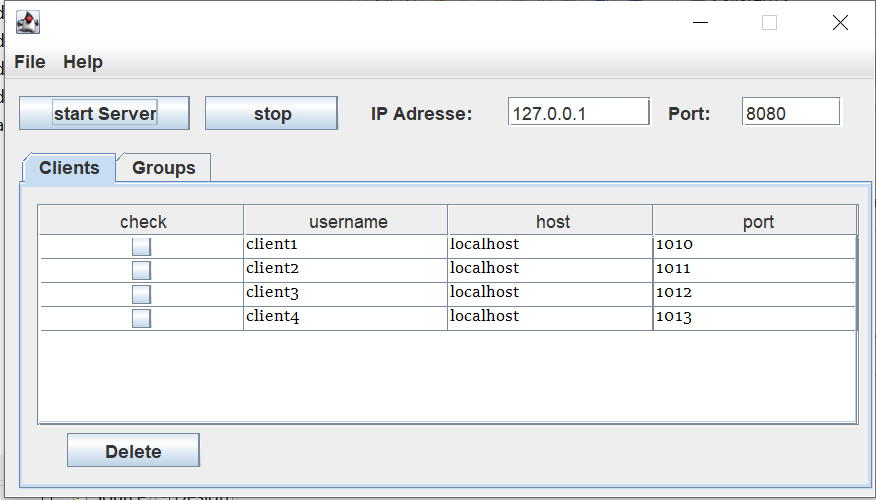
\includegraphics[width=0.7\textwidth]{gfx/GUI_Server_Clients}
    \caption{GUI-Server-Clients}
    \label{fig:gui-server-clients}
\end{figure}

\noindent
The "Groups" table has less columns than the "Clients" table, namely (Check, Name of the group,
count of clients ).
The "Check" column has the same principle of operation as in the "Clients " table, the groups
can be selected to be deleted.

\begin{figure}
    \centering
    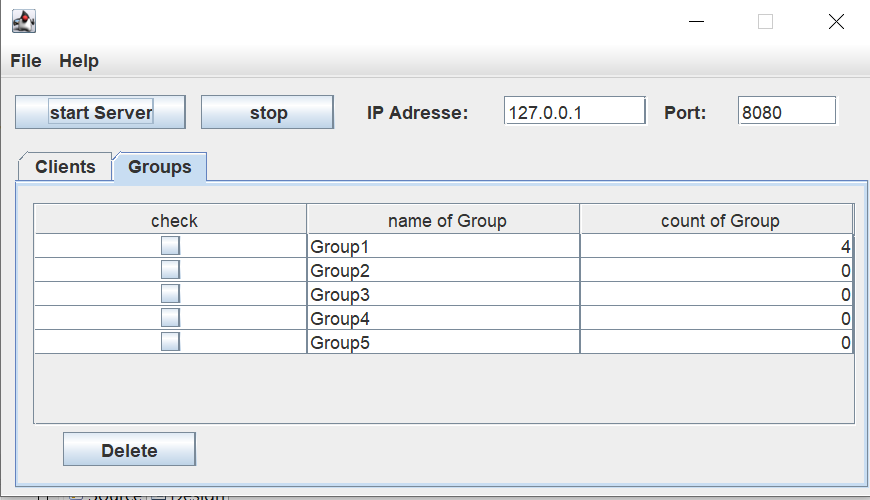
\includegraphics[width=0.7\textwidth]{gfx/GUI_Server_Groups}
    \caption{GUI-Server-Groups}
    \label{fig:gui-server-groups}
\end{figure}

\noindent
when a client is deleted, a message is sent to all other clients with the content
(the client is deleted with server).
This message \(the Group is deleted with serve\) is also sent for all clients when a group is deleted.
\medskip

\noindent
If you want to stop the server, it must click on the "Stop" button at the top of the mask.
when you want to close the server application, click on File -->Exit.

\section {Client GUI}\label{sec:client-gui}
There are two panels in the client interface, namely the configuration panel and the chat panel.
In the configuration panel you have to enter the ip address and port of the server but as default
values they are entered as follows ( IP-address :127.0.0.1 , port : 8080 ) After that the
IP-address and port of client is detected.
\medskip

\noindent
The username is set as default by "Client" and "Port" \( Example Username : Client65001\).
\begin{figure}
    \centering
    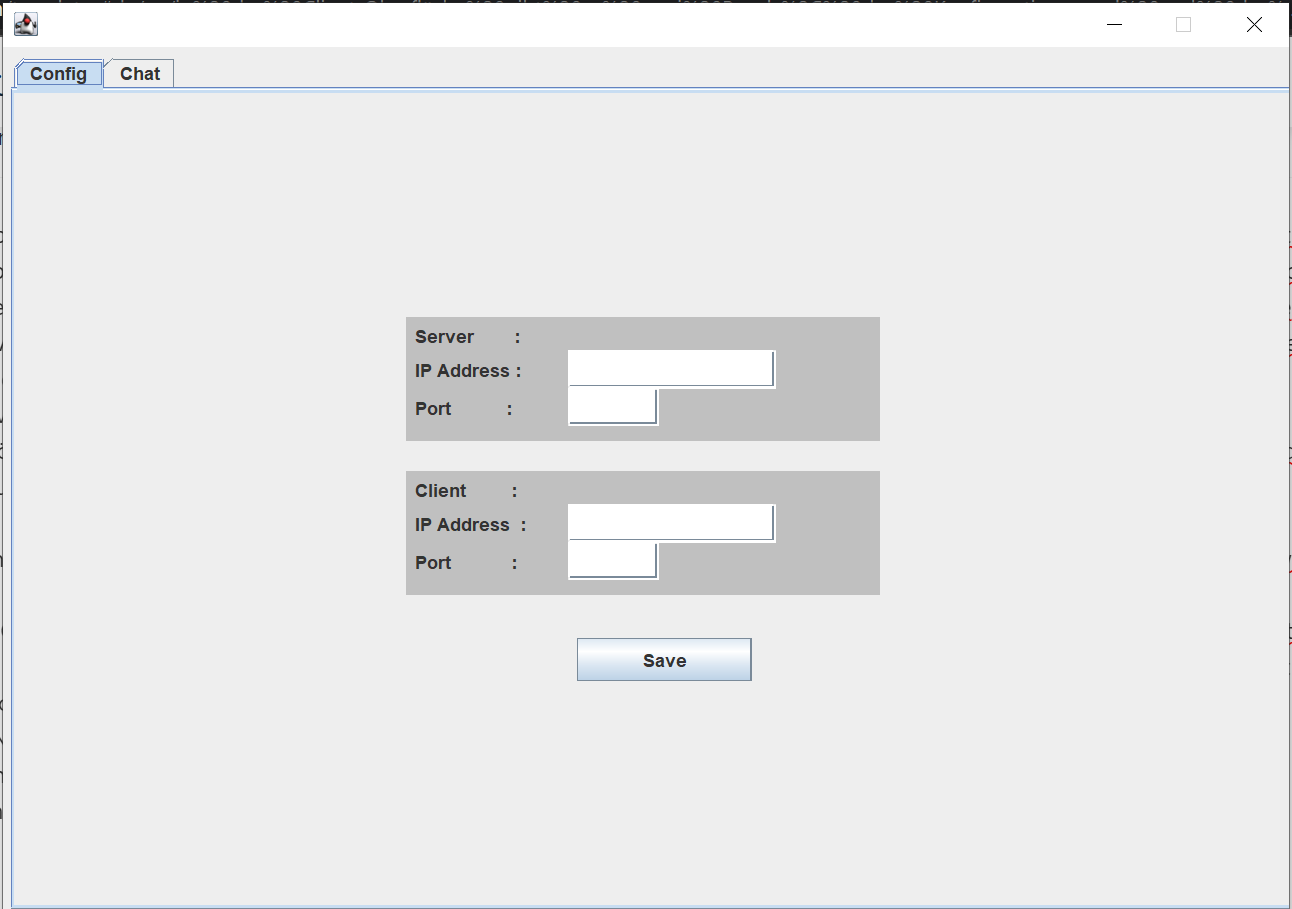
\includegraphics[width=0.7\textwidth]{gfx/Client_Config}
    \caption{Configuration of Client}
    \label{fig:Client-config}
\end{figure}
\noindent
After that you have to click on the Save button to start the client.
After adding the server and the client the configuration Panel will be displayed and chat Panal
will be enabled.
In the chat you can select contacts or groups so that the user can communicate with them.
The user can also create and join or left a group by himself.
If you want to see all clients and Groups , click the Search button
The chat panel shows all clients with that the user has written.
The messages between the clients are displayed and where the client can write.
The chat also has a button to send different files like video, image and audio.
\begin{figure}
    \centering
    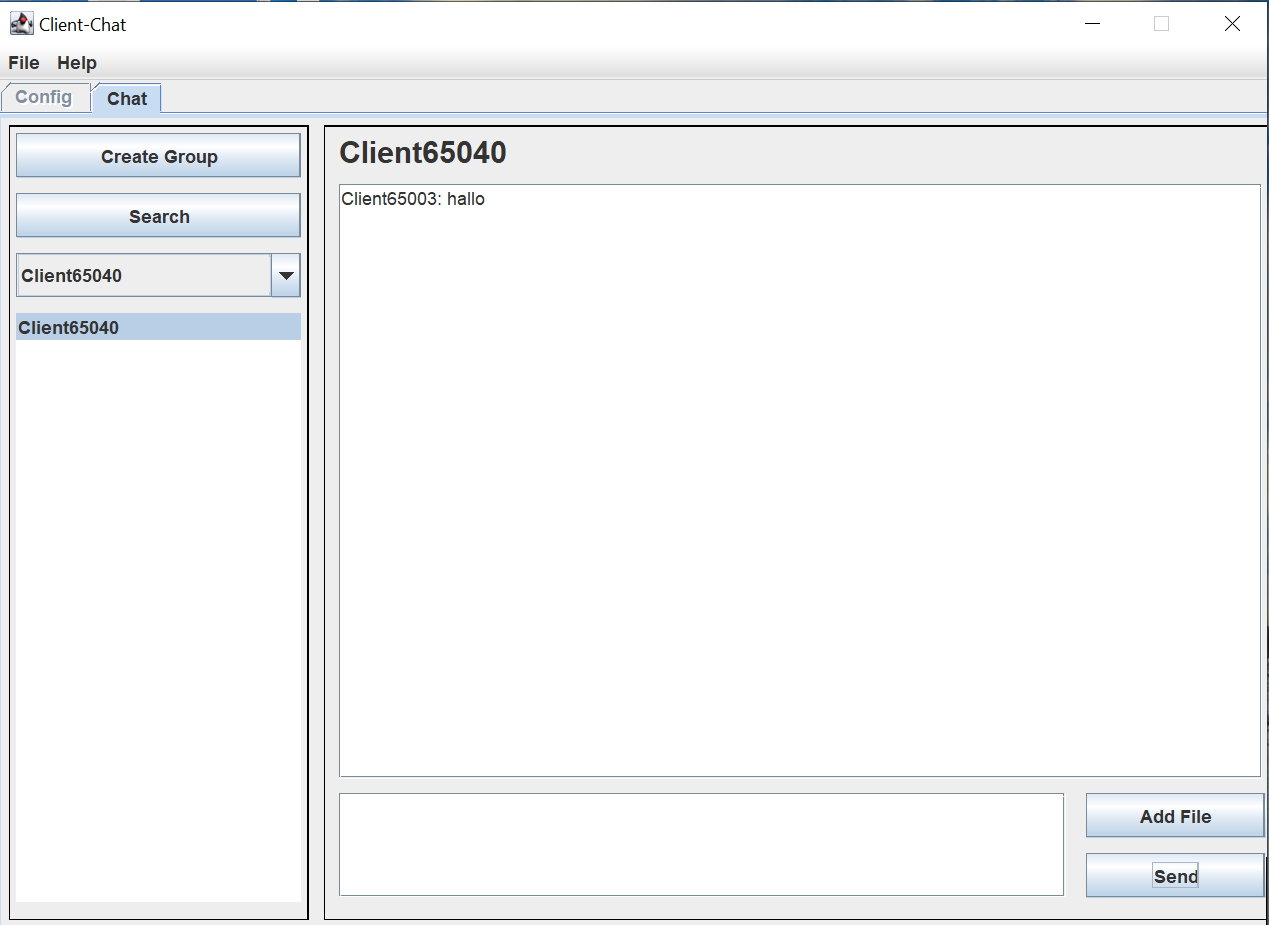
\includegraphics[width=0.7\textwidth]{gfx/Client_Chat}
    \caption{Chat of Client}
    \label{fig:Client-Chat}
\end{figure}

\section {Group}\label{sec:group}
When you click Create Group, a group is created on the server and displayed in a list
where you can see all the created groups and clients. In this list you can search for the group
you are looking for and find it quickly.
The client that created the group will be the first member added to the group.
Any client can create a group and then all other clients can join this group,
by clicking on the selected group.
When a client writes to the group or sends a file, all other clients see this file.
Any client can also leave the group at any time

\begin{figure}
    \centering
    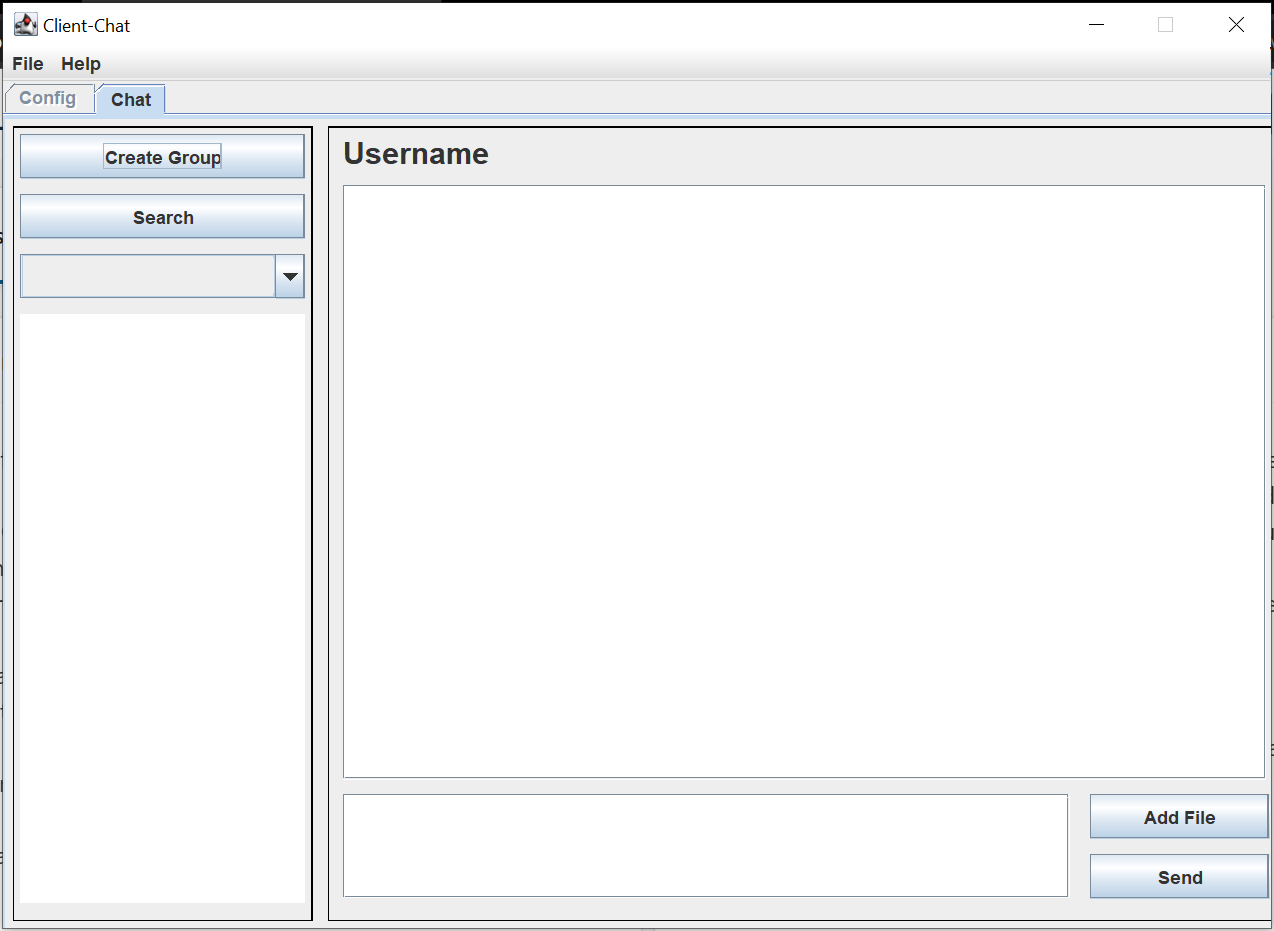
\includegraphics[width=0.7\textwidth]{gfx/Gruppe}
    \caption{Gruppe}
    \label{fig:Gruppe}
\end{figure}
